
\section{Overview}\label{subsec:overview}

We begin by considering the company structure introduced in Figure~\ref{company_structure}.

\begin{figure}[ht!]
\centering
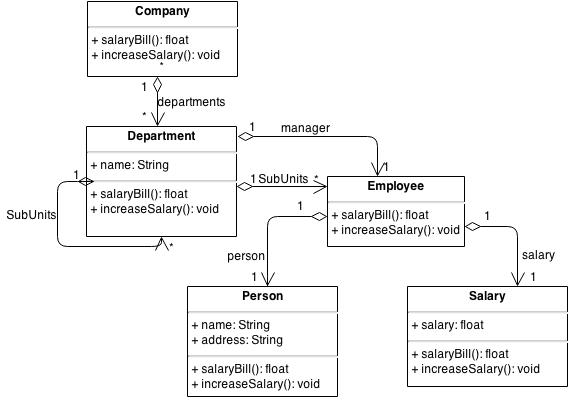
\includegraphics[width=90mm]{Company.jpg}
\caption{Company Structure \label{company_structure}}
\end{figure}

A company is divided into departments which in turn have a manager, and consists of a collection of sub-units. A unit is either a single employee or a department. Both managers and ordinary employees are persons receiving a salary. A common OOP programmer may organize the code like Figure~\ref{oop_company} and Figure~\ref{oop_salary}. Similar code can be applied to Department, Employee, SubUnit and Person. 

\begin{figure}[tb]
\lstinputlisting[linerange=6-17]{../ObjectAlgebras/src/sybDemo1/Company.java} % APPLY:linerange=OOP_COMPANY
\vspace{-.1in}
\caption{Company Class of OOP style}
\label{oop_company}
\end{figure}

\begin{figure}[tb]
\lstinputlisting[linerange=4-9]{../ObjectAlgebras/src/sybDemo1/Salary.java} % APPLY:linerange=OOP_SALARY
\vspace{-.1in}
\caption{Salary Class of OOP style}
\label{oop_salary}
\end{figure}

Now consider adding two operations to our company structure: query the salary bill for the whole company and increase the salary for the each employee by 10\%. The methods Float salaryBill() and void increaseSalary() in Figure~\ref{oop_company} and Figure~\ref{oop_salary} show an easy solution that an OOP programmer will possibly come up with. 

This way of OOP style representation of tree structures can become cumbersome and inflexible due to the bound relationship between classes. For example, adding a new operation such as pretty printing of the company structure requires a lot of changes on the existing code and violates the no modification rule. One can solve this problem by coding with object algebras as Figure~\ref{syb_tree}: 
\begin{figure}[tb]
\lstinputlisting[linerange=8-17]{../ObjectAlgebras/src/trees/SybAlg.java} % APPLY:linerange=SYB_TREE
\vspace{-.1in}
\caption{Company Structure represented by Object Algebra Interface}
\label{syb_tree}
\end{figure}

Hence different operations can be realized by inheriting object algebras from object algebra interface. Figure~\ref{query_salary} shows how to implement query salary operation based on the company algebra interface.  
\begin{figure}[tb]
\lstinputlisting[linerange=7-33]{../ObjectAlgebras/src/sybDemo2/SalaryQuerySybAlg.java} % APPLY:linerange=QUERY_SALARY
\vspace{-.1in}
\caption{Company Structure represented by Object Algebra Interface}
\label{query_salary}
\end{figure}

Increasing Salary is trickier. We need the visitable classes to help reconstruct  the tree structures. 
\begin{figure}[tb]
\lstinputlisting[linerange=6-8]{../ObjectAlgebras/src/sybDemo2/G_Company.java} % APPLY:linerange=G_COMPANY
\vspace{-.1in}
\caption{Generic Visitable Class of Company}
\label{g_company}
\end{figure}
\begin{figure}[tb]
\lstinputlisting[linerange=6-8]{../ObjectAlgebras/src/sybDemo2/G_Salary.java} % APPLY:linerange=G_SALARY
\vspace{-.1in}
\caption{Generic Visitable Class of Salary}
\label{g_salary}
\end{figure}
\begin{figure}[tb]
\lstinputlisting[linerange=9-67]{../ObjectAlgebras/src/sybDemo2/IncreaseSalarySybAlg.java} % APPLY:linerange=INCREASE_SALARY
\vspace{-.1in}
\caption{Increase Salary Class implementing Company Algebra Interface}
\label{increase_salary}
\end{figure}

However, although we solved the problem of extensibility with object algebras, the traversal code become so long and most of the time we are writing boilerplate routine code, which is to call the methods of its child leaves. The only code we are really interested in is the Salary S(Float salary) method to return the salary. It will be great if the boilerplate code can be generated automatically every time we want to traverse the tree structure. 

Motivated by this problem of generating generic code for tree structure traversals, more specifically, queries and transformations in object algebras, we designed an object algebra framework with great features. We introduce monoids in queries and generic visitable interfaces in transformations, and write generic query and transformation which can be easily inherited by real cases of queries and transformations. Furthermore, even the generic query and transformation code can be generated automatically by adding an ``$@$Algebra'' annotation. 

Now with our Object Algebra Framework, the code we need to write for Salary Bill and Increase Salary will be much shorter. A Generic query code will be as short as Figure~\ref{query_with_oaframework}. 
\begin{figure}[tb]
\lstinputlisting[linerange=7-12]{../ObjectAlgebras/src/test/FloatQuerySybAlgebra.java} % APPLY:linerange=QUERY_WITH_OAFRAMEWORK
\vspace{-.1in}
\caption{Query Salary Class with Object Algebra Framework}
\label{query_with_oaframework}
\end{figure}
Transformation code will be like Figure~\ref{transform_with_oaframework}
\begin{figure}[tb]
\lstinputlisting[linerange=7-15]{../ObjectAlgebras/src/transform/SybIncSalary.java} % APPLY:linerange=TRANSFORM_WITH_OAFRAMEWORK
\vspace{-.1in}
\caption{Increase Salary Class with Object Algebra Framework}
\label{transform_with_oaframework}
\end{figure}